% Template for ISBI paper; to be used with:
%          spconf.sty  - ICASSP/ICIP LaTeX style file, and
%          IEEEbib.bst - IEEE bibliography style file.
% --------------------------------------------------------------------------
\documentclass{article}
\usepackage{spconf,amsmath,graphicx,hyperref}

% Example definitions.
% --------------------
\def\x{{\mathbf x}}
\def\L{{\cal L}}

% Title.
% ------
\title{Inexact Graph Matching for Neuron Tracking in Calcium Imaging}
%
% Single address.
% ---------------
\name{K. V. Busum$^1$, W. D. Tracy$^2$, L. He$^2$, S. Gulyanon$^3$, and G. Tsechpenakis$^1$ \thanks{This work is supported by NSF/DBI [$\#$1252597]: `CAREER: Modeling the structure and dynamics of neuronal circuits in the \emph{Drosophila} larvae using image analytics' awarded to G. Tsechpenakis.} \vspace{-5pt}}
\address{\small{$^1$Computer and Information Science Department, Indiana University-Purdue University Indianapolis, USA;} \\
	\small{$^2$ Department of Biology, Indiana University, USA;} \\
	\small{$^3$Data Science and Innovation Program, Faculty of Science and Technology, Thammasat University, Thailand;} \vspace{-2pt} \\}
%
% For example:
% ------------
%\address{School\\
%	Department\\
%	Address}
%
% Two addresses (uncomment and modify for two-address case).
% ----------------------------------------------------------
%\twoauthors
%  {A. Author-one, B. Author-two\sthanks{Thanks to XYZ agency for funding.}}
%	{School A-B\\
%	Department A-B\\
%	Address A-B}
%  {C. Author-three, D. Author-four\sthanks{The fourth author performed the work
%	while at ...}}
%	{School C-D\\
%	Department C-D\\
%	Address C-D}
%
% More than two addresses
% -----------------------
% \name{Author Name$^{\star \dagger}$ \qquad Author Name$^{\star}$ \qquad Author Name$^{\dagger}$}
%
% \address{$^{\star}$ Affiliation Number One \\
%     $^{\dagger}$}Affiliation Number Two
%
\begin{document}
%\ninept
%
\maketitle
%
\begin{abstract}
In this work, we propose the novel neuron tracking method that handles the issue in calcium images using the inexact graph matching over a set of graphs, each representing the neuron morphology at a time step. The match is computed by minimizing the graph edit distance that incorporates the tissue deformation, local image feature, neuronal morphology, and local characteristics of neurons.
\end{abstract}
%
\begin{keywords}
neuron tracking, calcium images, graph matching, graph edit distance, A*-beamsearch
\end{keywords}
%
\section{Introduction}
\label{sec:intro}


In this neuron tracking problem \cite{Gulyanon2018a}, we are given the calcium image stack sequence, $\mathcal{I} = \{ \mathcal{I}^{(t)} \}$, where $t = 0,1,\dots,T$. To make the problem feasible, we require the initial morphology of the neuron, $\mathcal{G} = \{ V_\mathcal{G}, E_\mathcal{G} \}$.

\section{Definitions}
A \emph{graph} is denoted by $G = \{V, E\}$, where $V$ is the set of nodes (also called \emph{vertices}) and $E \subset V \times V$ (or $E \subset [V]^2$) is the set of edges (also known as lines) of graph $G$. 

The problem of \emph{inexact graph matching} (IGM) or error-tolerant/correcting GM is finding the mapping of nodes between two graphs that optimizes a certain affinity or distortion criterion, where nodes do not need to have a correspondence in another graph.

A commonly used measurement of affinity criterion is the \emph{graph edit distance} (GED) \cite{gao2010}. A graph can be transformed to another one by a finite sequence of graph edit operations. Each operation has a cost, which is defined differently in various algorithms. GED, $\delta (G_i, G_j)$, is defined by the least-cost graph edit operation sequence, $P$, that is needed to transform one graph, $G_i = \{V_i, E_i\}$, into another, $G_j = \{V_j, E_j\}$.

\begin{equation} \label{eq:ged}
\delta(G_i, G_j) = \min_P \sum_{(u \rightarrow v) \in P} c(u \rightarrow v)
\end{equation}
where nodes $u \in V_i$ and $v \in V_j$ are a correspondence; and $c(u \rightarrow v)$ is the cost of the graph edit operation that maps node $u$ to $v$, which depends on the affinity between $u$ and $v$.

\section{Method}
In this work, we tackle the neuron tracking problem over calcium images as the IGM problem computed by minimizing the GED.

Given the calcium image sequence, first convert every frame into the ``frame'' graph whose nodes are superpixels. Second, compute the ``template'' graph, which is the subgraph of the ``frame'' graph corresponded to the neuron trace, using the IGM. Finally, recover the trace by aligning every dendrite to the image cues, and repeat throughout the sequence (fig.~\ref{fig:method}).

\begin{figure}[b!]
	\centering
	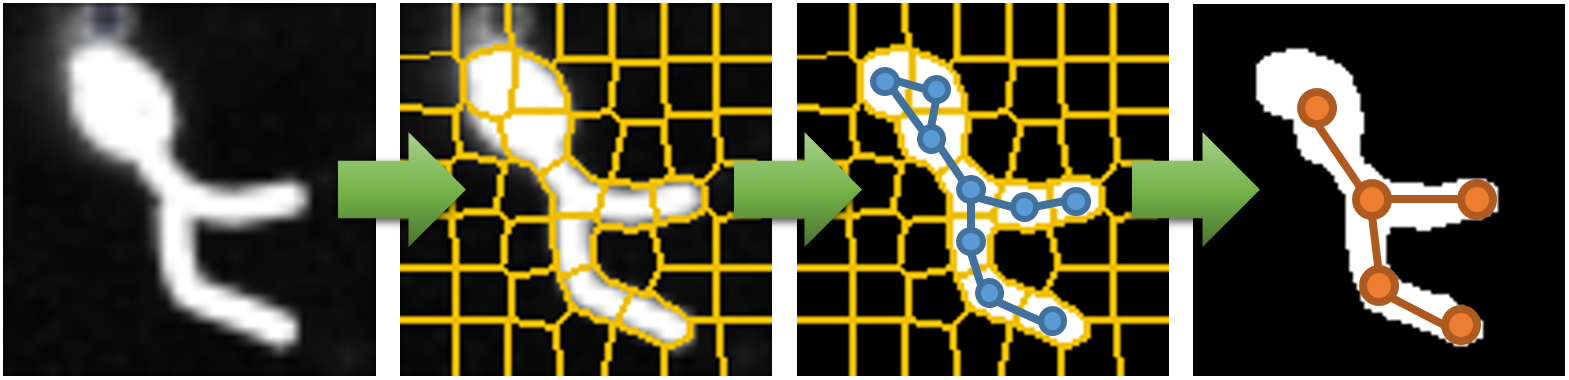
\includegraphics[width=\columnwidth]{img/method.png}
	\caption{\small{From left to right. Input image, the ``frame'' graph, the ``template'' graph, and the aligned neuron trace. Yellow lines show the boundary of superpixels. Blue color shows the ``template'' graph and orange colors shows the neuron trace result.}}
	\label{fig:method}
	\vspace{-10pt}
\end{figure}


\subsection{Creating ``Frame'' Graph}
Due to the imaging system limitation, the maximum intensity projection of calcium image stack, $I_t = f(\mathcal{I}^{(t)})$, is used instead of the raw input volume. 

To convert a frame into a graph, first compute the superpixel segmentation over $I_t$ using techniques like Linear Spectral Clustering Superpixel \cite{li2015, chen2017}\footnote{\url{https://jschenthu.weebly.com/projects.html},\\ \url{https://www.mathworks.com/matlabcentral/fileexchange/65684-linear-spectral-clustering-superpixel}} or simple linear iterative clustering (SLIC). The result is the set of superpixels $V_t$. 

Let the ``frame'' graph be $G_t = \{ V_t, E_t \}$, where the existence of edges $E_t$ between superpixels are computed using Delaunay triangulation over the centroids of superpixels in $V_t$.


\subsection{Initial ``Template'' Graph}
The trace describes the neuron morphology at the structural level, while the input image stacks describe the neuron at the appearance level. We propose the ``template'' graph that bridges between two levels of representations.

The ``template'' graph at time $t=0$, $G'_0 =  \{V'_0, E'_0 \}$, is the subgraph of $G_0$ corresponded to the initial morphology $\mathcal{G}$. $V'_0$ is the set of patches overlapping with $\mathcal{G}$, 
\begin{equation}
V'_0 = \{\,v \mid v \text{ overlaps } \mathcal{G}, v \in V_0 \,\}
\end{equation}
$E'_0$ is the set of edges between adjacent nodes in $V'_0$, 
\begin{equation}
E'_0 = \{\, (u, v) \mid (u, v) \in E_0 ;\; u, v \in V'_0 \,\}
\end{equation}


\subsection{Tree Search Algorithm} \label{sec:treealgo}
A tree (state space) search algorithm \cite{morrison2015} is used to find the GED because it is simple, allows the many-to-many mapping function, and makes no assumptions about the problem. Tracking is done by computing the GED between the previous ``template'' graph and the current ``frame'' graph, $\delta (G'_{t-1}, G_t)$. The tree state space consists of a number of possible mappings and the corresponding cost (fig.~\ref{fig:treesearch}). The algorithm terminates when every node in $G'_{t-1}$ has at least one correspondence in $G_t$.

%%TODO: add figure describing tree search algorithm
\begin{figure}[b!]
	\centering
	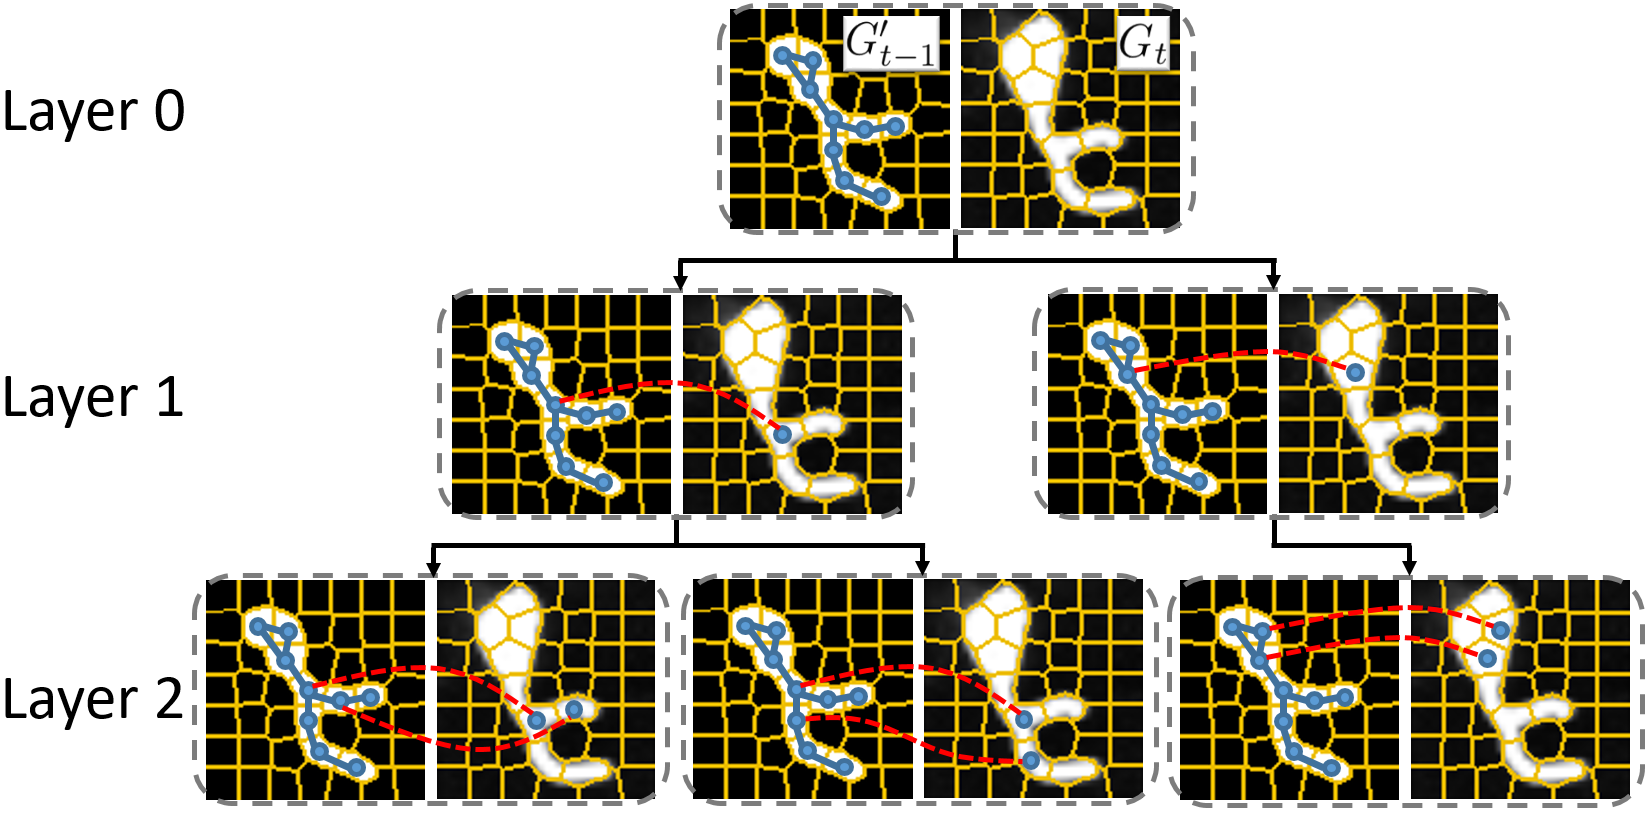
\includegraphics[width=\columnwidth]{img/treesearch.png}
	\caption{\small{Tree state space. The root of the state space represents the mapping with no correspondences. The first layer of states represents mappings with one correspondence, and so on. Red lines show pairs of nodes that are a correspondence.}}
	\label{fig:treesearch}
	\vspace{-10pt}
\end{figure}

A state is produced by adding a new correspondence to the parent state. Let $\psi$ be a function that determines, for a given state/mapping $p$, a set of possible new correspondences that can be added to form new child states. 
\small
\begin{equation}
\psi(p) = \{ \check{V}_{p,t-1} \times \check{V}_{p,t} \} \cup \{ \check{V}_{p,t-1} \times V_{p,t} \} \cup \{ V_{p,t-1} \times \check{V}_{p,t} \}
\end{equation}
\normalsize
where $\check{V}_{p,t}$ is the set of nodes that are not currently mapped and are adjacent to the set of mapped nodes $V_{p,t}$, $\check{V}_{p,t} = \{\, v \mid (u,v) \in E_t, u \in V_{p,t}, v \notin V_{p,t} \,\}$.



\subsection{Coarse Tracking}
Let $P$ be the graph edit operation sequence with the optimal GED; and $P(V_t)$ denotes the set of nodes $V_t$ mapped by the sequence $P$. Then, the ``template'' graph at time $t$ is defined by $G'_t =  \{V'_t, E'_t \}$, where
\begin{equation}
V'_t = P(V_t)
\end{equation}
And $E'_t$ is the set of edges between adjacent nodes in $V'_t$, 
\begin{equation}
E'_t = \{\, (u, v) \mid (u, v) \in E_t ;\; u, v \in V'_t \,\}
\end{equation}


\subsection{Fine Tracking: Aligning Dendrites}
Consider a set of vertices, $V_d \subset V_\mathcal{G}$, that constitutes a dendrite/branch $d$ in the neuron trace. The nodes corresponding to the dendrite $d$ in the ``template'' graph at time $t = 0$ is
\begin{equation}
V'_{d,0} = \{\,v \mid v \text{ overlap with } V_d, v \in V_0 \,\}
\end{equation}

For time $t$,
\begin{equation}
V'_{d,t} = P( V'_{d,t-1})
\end{equation}

The alignment between dendrite at consecutive time step is done by registering patches from $V'_{d,t-1}$ to $V'_{d,t}$ using techniques like free-form deformation (FFD) \cite{Rueckert1999}.


\section{Optimization}
A tree search algorithm in Section~\ref{sec:treealgo} that explores the whole state space is inefficient because the size of the state space is $|V'_{t-1}||V_t|$ and many states have no meaningful interpretation, e.g., mappings that produce unconnected dendrites. 

In this work, the computation of GED is improved by using the A*-beamsearch \cite{neuhaus2006} with node grouping, that only explores the most likely and meaningful states and allows many-to-many mapping solution.

\subsection{A* Search}
The A* or the best-first search algorithm \cite{hart1968} finds an optimal path from a state space based on a heuristic function, which estimates the expected costs of the best route from the root through the current state (partial solution) to a leaf state (complete solution). At each step during tree state space traversal, the most promising state --- the lowest heuristic cost --- from the set of child states is chosen. Hence, at any state $p$, A* algorithm selects the path that minimizes the following cost:
\begin{equation} \label{eq:a*}
f(p) = g(p) + h(p)
\end{equation}
where $g(p)$ is the cost of the optimal path from the root to the current state $p$ and $h(p)$ is the estimated cost from state $p$ to a leaf state. Here, $h(p)$ is defined by the average cost of $g(p)$ times the number of remaining unmapped nodes.

\subsection{Beam Search}
In A* search, we may end up expanding all successor nodes in the search tree. In beam search, only a fixed number, $b$ called \emph{beam width}, of states in each layer are explored. We pick the $b$ states with the lowest costs from eq.~\ref{eq:a*}. 

This means only those states with the most promising partial mappings are explored. Since a graph edit operation sequence between similar graphs has lower cost than the one between dissimilar graphs \cite{neuhaus2006}.



\section{Cost Function}
The cost function, $c(u \rightarrow v)$, of the GED $\delta (G'_{t-1}, G_t)$ takes a correspondence and returns a single value measuring its similarity based on the tissue deformation, local image feature, neuronal morphology, and local characteristics of neurons.

Edge comparison is not meaningful here since edge captures the relationship between nodes but the correspondent nodes are not guaranteed to be the same. However, we still need the neighborhood information that edges have. Thus, we aggregate the edge descriptors and embed them in the node descriptor. Next, we describe the cost function between two nodes (one-to-one function) and between a node and a group of nodes (many-to-one/one-to-many functions)

\subsection{Node to Node}
\textbf{Average intensity} of any node $v_i \in V_t$ is defined by,
\begin{equation}
I_t(v_i) = \frac{1}{|S(v_i)|}\sum_{x \in S(v_i)} I_t(x)
\end{equation} 
where $S(v_i)$ is the set of pixels in the superpixel corresponded to node $v_i$.

\textbf{Average eigenvector} from Frangi filter \cite{frangi1998} indicates the neurite orientation,
\begin{equation}
F(v_i) = \frac{1}{|S(v_i)|}\sum_{x \in S(v_i)} \hat{\textbf{u}}_{x,1}
\end{equation}
where Let $\lambda_{s,x,k}$ denote the eigenvalue corresponding to the $k$-th normalized eigenvector $\hat{\textbf{u}}_{s,x,k}$
of the Hessian matrix of the image $\mathcal{H}_{x,k}$ all computed at scale $s$ on pixel $x$. 
\begin{equation}
\lambda_{x,k} = \max_{s_{min} \le s \le s_{max}} \lambda_{s,x,k}
\end{equation}
will be the eigenvalue with the $k$-th smallest magnitude ($\lambda_{x,1} < \lambda_{x,2}$) and $\hat{\textbf{u}}_{x,k}$ are their corresponding eigenvectors.

\textbf{Relation to neighbors} measures the intensity similarity between a node and its neighborhood. To compute, first find the location $L_{ij}$ and magnitude $M_{ij}$ based on the average intensity similarity for each neighbor $v_j$ of $v_i$, $(v_i, v_j) \in E_t$,
\begin{equation}
\begin{aligned}
L_{ij} & = C(v_j) - C(v_i) \\
M_{ij} & = 1 - \| I_t(v_j) - I_t(v_i) \|
\end{aligned}
\end{equation}
where $C(v_i)$ is the centroid of the superpixel corresponded to node $v_i$ denoted by the $xy$-coordinate, $(x_i, y_i)$.

Then, a histogram is created to encode the relation to neighboring superpixels, similar to the orientation histogram in SIFT \cite{lowe1999}. In this histogram, the 360 degrees of $L_{ij}$ direction are broken into 8 bins (each 45 degrees). The amount added to the bin depends on the magnitude projected in the bin's direction.

To achieve rotation independence, make the orientation relative to the keypoint's orientation by subtracting the keypoint's rotation from each orientation. The keypoint is the bin with the highest magnitude.

To achieve illumination dependence, threshold the magnitudes that are too big.

Similarly, \textbf{relation to mapping} indicates the proximity between $v_i$ and mapped nodes. This helps distinguish nodes along ambiguous regions like dendrites since points along the dendritic line segment have similar properties. It is a histogram of mapped neighbors' orientation weighted by the inverse of distance $H_{ij}$, where $v_j \in V_{p,t}$.
\begin{equation}
H_{ij} = \frac{1}{ \| L_{ij} \| }
\end{equation}

\textbf{Smooth deformation} keeps the change in deformation low over space. For $u_i^{t-1} \in \check{V}_{p,t-1}$ and $v_i^t \in \check{V}_{p,t}$, the deformation of the correspondence $i$ is defined as,
\begin{equation}
d_i = C(u_i^{t-1}) - C(v_i^t)
\end{equation}

For $(u_i^{t-1}, u_j^{t-1}) \in E'_{t-1}$ and $(v_i^t, v_j^t) \in E_t$, where $u_i^{t-1}$ and $v_i^t$ are correspondence we are considering; $u_j^{t-1} \in V_{p,t-1}$ and $v_j^t \in  V_{p,t}$ are the adjacent correspondences we found earlier. Then, the change in deformation at correspondence $i$ is:
\begin{equation}
D_i = \sum_{d_j} \| d_j - d_i \|
\end{equation}

Hence, the node descriptor $\alpha(v_i)$ is defined as the tuple of 19 numbers: average intensity $I_t(v_i)$, the orientation of the average eigenvector $F(v_i)$ in radian, smooth deformation $T_i$, and the values in both histograms' bins.

The cost of substituting node $(u,v) \in \{ \check{V}_{p,t-1} \times \check{V}_{p,t} \}$ is defined based on cosine similarity as follows:
\begin{equation}
c(u \rightarrow v) = 1 - \frac{\sum_{i=1}^N \alpha_i(u)\alpha_i(v)}{\sqrt{\sum_{i=1}^N \alpha_i^2(u)}\sqrt{\sum_{i=1}^N \alpha_i^2(v)}}
\end{equation}

\subsection{Node to Group of Nodes}
The node grouping is needed for finding many-to-many relationship between frames in an efficient way, similar to \cite{morrison2015}.

The cost of substituting node $(u,v) \in \{ \check{V}_{p,t-1} \times V_{p,t} \}$ is defined based on cosine similarity as before but the labeling function of $u$ must take into account other correspondences of $v$.

Let $\hat{u}$ is the set of nodes correspondence to $v$, $\hat{u} = \{\, w \mid (w \rightarrow v) \in p \,\} \cup \{u\}$. Then, $\alpha(\hat{u})$ denotes the group-of-node descriptor. \textbf{Average intensity} and \textbf{average eigenvector} of a group of nodes are defined as,
\begin{equation}
\begin{aligned}
I_t(\hat{u}) & = \frac{1}{|S(\hat{u})|}\sum_{x \in S(\hat{u})} I_t(x) \\
F(\hat{u}) & = \frac{1}{|S(\hat{u})|}\sum_{x \in S(\hat{u})} \hat{\textbf{u}}_{x,1}
\end{aligned}
\end{equation} 

The \textbf{relation to neighbors} and \textbf{relation to mapping} are quantified from the neighbors of the group of nodes, ignoring the internal edges within the group. Using the centroid of the group of nodes and edges between a group of nodes and other nodes.

The cost of substituting node $(u,v) \in \{ V_{p,t-1} \times \check{V}_{p,t} \}$ follows the same suit.






\section{Results}


\section{Conclusion}

% To start a new column (but not a new page) and help balance the last-page
% column length use \vfill\pagebreak.
% -------------------------------------------------------------------------
\vfill
\pagebreak


% References should be produced using the bibtex program from suitable
% BiBTeX files (here: strings, refs, manuals). The IEEEbib.bst bibliography
% style file from IEEE produces unsorted bibliography list.
% -------------------------------------------------------------------------
\bibliographystyle{IEEEbib}
\small{
\bibliography{all}
%\begin{thebibliography}{10}
%	
%\bibitem{Gulyanon2018a}
%S.~Gulyanon, L.~He, W.D. Tracey, and G.~Tsechpenakis,
%\newblock ``Neurite tracking in time-lapse calcium images using {MRF}-modeled
%pictorial structures,''
%\newblock in {\em ISBI}, 2018, pp. 1564--1568.
%
%\bibitem{gao2010}
%X.~Gao, B.~Xiao, D.~Tao, and X.~Li,
%\newblock ``A survey of graph edit distance,''
%\newblock {\em Pattern Anal Appl}, vol. 13, no. 1, pp. 113--129, 2010.
%
%\bibitem{li2015}
%Z.~Li and J.~Chen,
%\newblock ``Superpixel segmentation using linear spectral clustering,''
%\newblock pp. 1356--1363, 2015.
%
%\bibitem{chen2017}
%J.~Chen, Z.~Li, and B.~Huang,
%\newblock ``Linear spectral clustering superpixel,''
%\newblock {\em IEEE Trans Image Process}, vol. 26, no. 7, pp. 3317--3330, 2017.
%
%\bibitem{neuhaus2006}
%M.~Neuhaus, K.~Riesen, and H.~Bunke,
%\newblock ``Fast suboptimal algorithms for the computation of graph edit
%distance,''
%\newblock pp. 163--172, 2006.
%
%\bibitem{hart1968}
%P.~Hart, N.~Nilsson, and B.~Raphael,
%\newblock ``A formal basis for the heuristic determination of minimum cost
%paths,''
%\newblock {\em IEEE transactions on Systems Science and Cybernetics}, vol. 4,
%no. 2, pp. 100--107, 1968.
%
%\bibitem{frangi1998}
%A.F. Frangi, W.J. Niessen, K.L. Vincken, and M.A. Viergever,
%\newblock ``Multiscale vessel enhancement filtering,''
%\newblock pp. 130--137, 1998.
%
%\bibitem{lowe1999}
%D.G. Lowe,
%\newblock ``Object recognition from local scale-invariant features,''
%\newblock {\em ICCV}, vol. 99, no. 2, pp. 1150--1157, 1999.
%
%\bibitem{morrison2015}
%P.~Morrison and J.J. Zou,
%\newblock ``Inexact graph matching using a hierarchy of matching processes,''
%\newblock {\em Computational Visual Media}, vol. 1, no. 4, pp. 291--307, 2015.
%
%\bibitem{Rueckert1999}
%D.~Rueckert, L.I. Sonoda, C.~Hayes, D.L.G. Hill, M.O. Leach, and D.J. Hawkes,
%\newblock ``Nonrigid registration using free-form deformations: Application to
%breast {MR} images,''
%\newblock {\em IEEE Trans Med Imag}, vol. 18, no. 8, pp. 712--721, 1999.
%	
%\end{thebibliography}
}

\end{document}
